\documentclass[12pt, oneside]{article}   	% use "amsart" instead of "article" for AMSLaTeX format
\usepackage{geometry}                		% See geometry.pdf to learn the layout options. There are lots.
\geometry{letterpaper}                   		% ... or a4paper or a5paper or ... 
%\geometry{landscape}                		% Activate for for rotated page geometry
%\usepackage[parfill]{parskip}    		% Activate to begin paragraphs with an empty line rather than an indent
\usepackage{graphicx}				% Use pdf, png, jpg, or eps§ with pdflatex; use eps in DVI mode
								% TeX will automatically convert eps --> pdf in pdflatex		
\usepackage{amssymb}
\usepackage{mathtools}
\usepackage{setspace}
\title{Conference Grant Proposal: ``Children Use Phonetically-Cued Talker Information to Infer Speaker Meaning"}
\author{Nicholas P. Moores \\ Department of Linguistics, Stanford University}
\date{}							% Activate to display a given date or no date

\begin{document}
\maketitle
%\section{}
%\subsection{}
\section{Revisions Since Last Submission} Professor Sumner has now sent in her letter of support for my receiving this conference grant. Thank you so much for your patience and diligence.
\section{Proposal Title} {\bf Children use phonetically-cued talker information to infer speaker meaning}
\section{Conference Abstract} 

Speech perception provides an avenue with which to study children's burgeoning ability to comprehend social information in the speech stream. The speech signal contains not only phonemic information necessary for word recognition but abundant indexical information about the talker, including talker gender (Perry, Ohde, \& Ashmead, 2001; Goldinger, 1998; Johnson et al., 1999; Johnson, 2006). A growing body of work has begun to investigate the effects of listeners' associations between talkers' social identity and the phonetic cues in talkers' voices, demonstrating that by adulthood listeners use talker information to make social inferences about a talker's likely behavior (Van Berkum et al., 2008), especially when they expect talker identity to be useful or find it to be a reliable cue (Creel, Aslin, \& Tanenhaus, 2008). Recent work suggests that children use acoustic cues to talker identity to constrain
comprehension of spoken language (Creel, 2012), though the way in which children learn to integrate social knowledge with information from talker voice remains poorly understood. In this paper, we test the hypothesis that
children are able to disambiguate between objects with gendered associations (a men's pair of gloves and a women's pair of gloves, say) based on talker voice. We explore children's use of talker indexical information to infer speaker meaning through an experiment in which children interact with a web page on an iPad. Over 24 trials, children ages 3-5 were shown series of four images and asked by talkers to find one of the objects by clicking on it. During half of the trials, children heard a male talker's voice, and during the other half they heard a female talker's voice. In addition, half of the trials were non-competitor trials in which there was only one image of the talker's referent (hearing a man's voice and seeing a man's glove, say). The other half were competitor trials in which the target image competed with a variant which would stereotypically belong to a speaker of the opposite gender (hearing a man's voice but choosing between both a man's glove and a woman's glove). Children's reaction time between the utterance of the target word and their click on an image was logged, as was their choice of image. Our data suggest that by the age of 5, children regularly integrate phonetically-cued socially indexical talker information with their social knowledge of speaker characteristics to guide their interpretations of speaker meaning in a real world paradigm. From ages 3 to 5, the ability to disambiguate increases significantly. All ages are extremely good at the task in non-competitor trials. Interestingly, in competitor trials, as age increases, children are faster and more accurate in disambiguating the voice cues. These results suggest not only that children make use of socially-nuanced talker-specific acoustic information by a young age, but reveal a robust understanding of gender stereotypes that guide their daily interactions with interlocutors and may bear on their linguistic and social development.

\begin{figure}[h!]
  \centering
    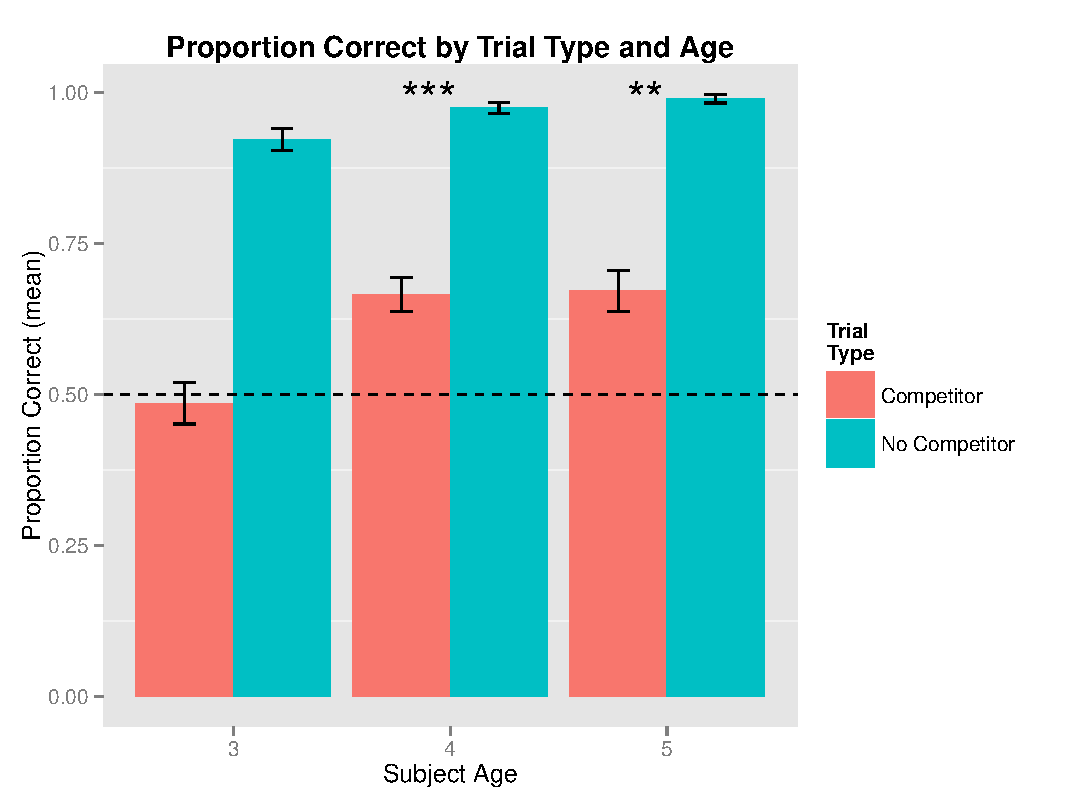
\includegraphics[width=1.2\textwidth]{CLAV_Exp1_ProportionCorrect.pdf}\
    \caption{Four-year-olds ($\beta=0.79$, $SE=0.18$, $z=2.794$, $p < 0.01$) and five-year-olds ($\beta=1.10$, $SE=0.32$, $z=3.406$, $p < 0.001$) significantly improved over three-year-olds; girls significantly better than boys in the task ($\beta=0.76$, $SE=0.24$, $z=3.101$, $p = 0.002$)}
\end{figure}

\begin{figure}[h!]
  \centering
    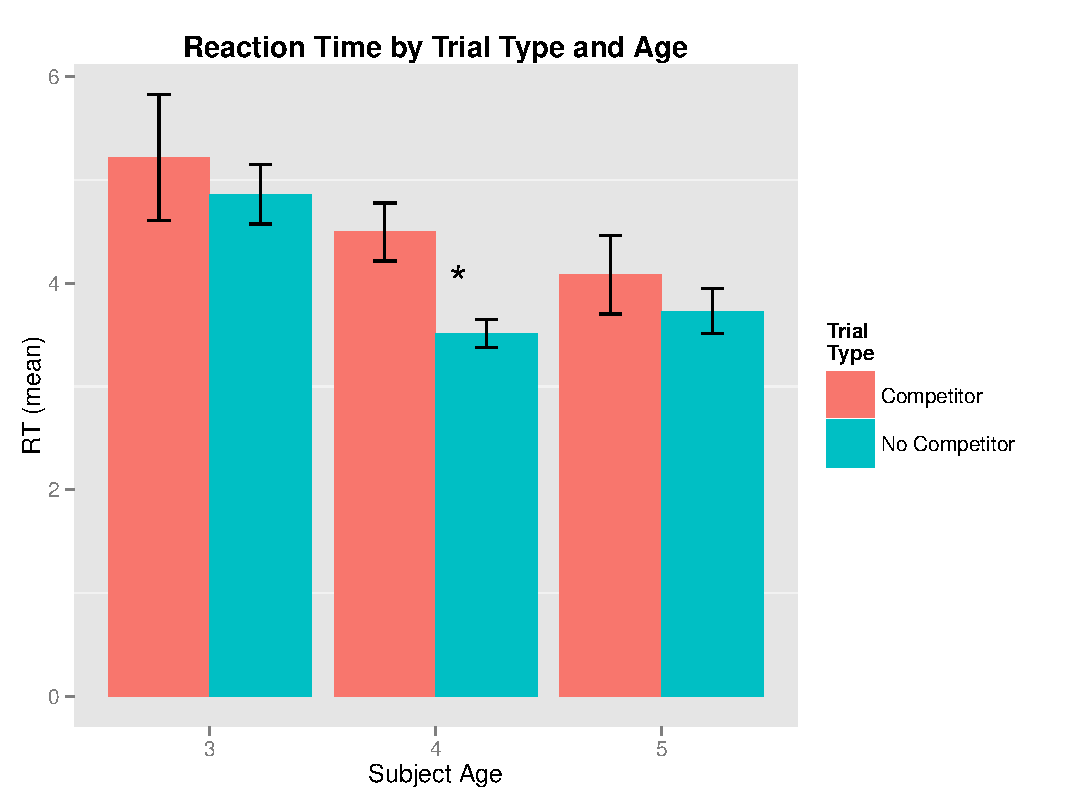
\includegraphics[width=1.2\textwidth]{CLAV_Exp1_MeanRT.pdf}\
    \caption{Mean Reaction Time by Age; no significant difference by age or gender}
\end{figure}
\section{Applicant's Role in the Presentation} I will be personally leading the poster presentation on my research. Although I have co-authors, I will be solely responsible for presenting and responding to questions from the audience.
\section{Conference to Attend} The conference I will be attending is The 89th Annual Meeting of the Linguistic Society of America in Portland, Oregon. The conference will take place from January 8 through January 11, 2015. I am approved to present in the Saturday Morning Plenary Poster Session (Saturday, January 10 from 10:30AM - 12:00 PM. I received the following abstract acceptance notification on September 16, 2014:

{\it Dear Nicholas Moores,

We are pleased to inform you that the LSA Program Committee has accepted your abstract for presentation as a poster at the Society's Eighty-ninth Annual Meeting, to be held 8-11 January, 2015 in Portland, Oregon. This year we considered 491 submissions as candidates for poster presentations. We accepted 150 of these submissions, for an acceptance rate of 30.55\%. If you indicated "paper" as your first-choice format and "poster" as your second-choice format, this means that your presentation has been assigned to the latter format, and we have changed the "submission type" fields on your abstract accordingly.

The Program Committee has scheduled plenary poster sessions on Friday and Saturday morning, January 9 and 10 in the Exhibit Hall on the Ballroom Level of the Hilton Portland \& Executive Tower. Posters will be on display from 9:00 AM to 5:00 PM, and every poster has been assigned to an attended session of 90 minutes, from 10:30 AM to 12:00 Noon on either Friday or Saturday. Poster presenters are expected to be available to answer questions at their poster during their assigned session. Beginning on Wednesday, September 17, you will be able to see the date, time, and name of the session to which your abstract has been assigned by logging in to the LSA website and clicking on the ?My Abstracts? link. The 100-word short abstract you submitted will be used in producing the Annual Meeting Handbook and in the online meeting guide.

Each poster presenter will be provided with a 4 x 8 ft. horizontal poster board and push pins. For those of you unfamiliar with what one looks like, a photo of a representative poster board may be found at http://www.linguisticsociety.org/files/posterboard.jpg. A helpful publication entitled ""How to Design and Present a Successful Poster"" may be found at http://www.linguisticsociety.org/resource/lsa-poster-guidelines. Note that Wi-Fi internet access may not be available in the foyer where the posters are displayed.

If you will be presenting your poster in ASL and will need sign language interpretation, please let me know no later than October 1 (drobinson@lsadc.org) so we can make appropriate arrangements for an interpreter.

If you must withdraw your poster from the 2015 Annual Meeting, please let us know no later than October 1.

On the day of your attended session, you are expected to put your poster up between 8:00 and 9:00 AM, and to remove it between 5:00 PM and 6:00 PM. Authors are encouraged to provide handouts for their papers. Please bring sufficient copies of your handout for distribution, and remember that the LSA will not be able to make additional copies of your handouts for you; the hotel's business center may be used for this purpose.

More information, including links to Annual Meeting preregistration (available through from October 1 through December 19) and online hotel reservations (available through December 6) is available at http://www.linguisticsociety.org/event/lsa-2015-annual-meeting. Please note that all individuals attending the meeting are expected to register for it.

Presenters of papers and posters at the 2015 Annual Meeting will also be strongly encouraged to submit extended abstracts for publication on the LSA website. We will contact you later with further instructions should you wish to submit an extended abstract.

We look forward to seeing you next January.

Sincerely,

Molly Diesing
Marlyse Baptista
Co-Chairs, Program Committee
Linguistic Society of America

Title: Children use phonetically-cued talker information to infer speaker meaning
Link: http://www.linguisticsociety.org/abstract/children-use-phonetically-cued-talker-information-infer-speaker-meaning}

\section{Process by which I was Accepted} My abstract was accepted after going through a competitive peer-reviewed selection process.
\section{Goals of Attending the Conference} I will attend the sessions on speech perception, experimental phonetics, psycholinguistics, language acquisition, and experimental pragmatics, and hope to talk to faculty presenting in each of these subfields about their research and how I believe my interests and theirs are aligned. By attending LSA 2015, I hope to learn about the cutting-edge work being done by researchers in each of these subfields. If I were not able to attend this conference, I would not be able to simultaneously be exposed to advanced research in each of these subfields, let alone discuss the role of these works within their own fields and in other related fields with the actual researchers conducting this work. Attending LSA 2015 will provide me with a fantastic and invaluable opportunity to deepen my connections with the broader linguistics community, be exposed to work in other subfields related to my own, and to be able to see my own work in the context of contemporary work across the subfields of linguistics being conducted at other research institutions. Importantly, attending LSA will allow me not only to get further depth in fields of linguistics I am interested in, but will allow me to develop new interests that I otherwise might not have been exposed to.
\section{Budget} The requested budget for this project is \$950.
\begin{enumerate}
\item Lodging at Hotel Reserved for Conference Attendees (3 nights at the Hilton Portland and Executive Tower at \$120 per night): \$360.
\item Roundtrip Flight from San Francisco to Portland (two flights with checked baggage): \$390.
\item Conference Registration, student rate: \$70.
\item Membership Fee (necessary for acceptance to conference): \$40.
\item Food: \$90.
\item Total Funds: \$950.
\end{enumerate}
\end{document}  